%%%%%%%%%%%%%%%%%%%%%%%%%%%%%%%%%%%%%%%%%%%%%%%%%%%%%%%%%%%%%%%%%%%%%%%

\chapter{Experiment 4: Real-Time Clock Applications}

This chapter presents the implementation of a Real-Time Alarm Clock using Arduino UNO, a DS1307 RTC module, an SSD1306 OLED display, push buttons, and a buzzer. The project demonstrates real-time clock interfacing, alarm setting, user interaction through push buttons, and embedded timing applications.

%%%%%%%%%%%%%%%%%%%%%%%%%%%%%%%%%%%%%%%%%%%%%%%%%%%%%%%%%%%%%%%%%%%%%%%

\section{Real-Time Alarm Clock Using RTC and OLED Display}

%%%%%%%%%%%%%%%%%%%%%%%%%%%%%%%%%%%%%%%%%%%%%%%%%%%%%%%%%%%%%%%%%%%%%%%

\subsection{Project Name}

Real-Time Alarm Clock Using Arduino UNO, DS1307 RTC Module, SSD1306 OLED Display and Push Buttons

%%%%%%%%%%%%%%%%%%%%%%%%%%%%%%%%%%%%%%%%%%%%%%%%%%%%%%%%%%%%%%%%%%%%%%%

\subsection{Problem Statement}

The objective of this project is to interface a DS1307 Real-Time Clock (RTC) module with Arduino UNO using the I\textsuperscript{2}C communication protocol and display the current date and time on an SSD1306 OLED display.

The system also provides an alarm-setting mechanism using push buttons. Users can configure the alarm hour, minute, and second through dedicated buttons. When the current RTC time matches the preset alarm time, the buzzer is continuously activated until the time changes.

%%%%%%%%%%%%%%%%%%%%%%%%%%%%%%%%%%%%%%%%%%%%%%%%%%%%%%%%%%%%%%%%%%%%%%%

\subsection{Components Used \& Pin Connections}

\begin{table}[H]
\centering

\begin{minipage}[t]{0.48\textwidth}
\centering
\caption{Alarm Clock Components}
\label{tab:alarm_components}

\begin{tabular}{|p{4cm}|c|}
\hline
\textbf{Component} & \textbf{Quantity} \\
\hline
Arduino UNO & 1 \\
DS1307 RTC Module & 1 \\
SSD1306 OLED Display & 1 \\
Push Buttons & 3 \\
Buzzer & 1 \\
Breadboard & 1 \\
Jumper Wires & Required \\
\hline
\end{tabular}

\end{minipage}
\hfill
\begin{minipage}[t]{0.47\textwidth}
\centering
\caption{Push Button Connections}
\label{tab:alarm_buttons}

\begin{tabular}{|c|c|p{3cm}|}
\hline
\textbf{Button} & \textbf{Pin} & \textbf{Function} \\
\hline
P-adj & D1 & Change Alarm Setting Mode \\
P+ve & D2 & Increase Value \\
P-ve & D3 & Decrease Value \\
\hline
\end{tabular}

\end{minipage}

\end{table}

%%%%%%%%%%%%%%%%%%%%%%%%%%%%%%%%%%%%%%%%%%%%%%%%%%%%%%%%%%%%%%%%%%%%%%%

\subsection{RTC, OLED and Buzzer Connections}

\begin{table}[H]
\centering
\caption{RTC, OLED and Buzzer Connections}
\label{tab:alarm_connections}

\begin{tabular}{|l|c|}
\hline
\textbf{Device} & \textbf{Arduino Pin} \\
\hline
Buzzer (+) & D12 \\
Buzzer (-) & GND \\
RTC VCC & 5V \\
RTC GND & GND \\
RTC SDA & A4 \\
RTC SCL & A5 \\
OLED VCC & 5V \\
OLED GND & GND \\
OLED SDA & A4 \\
OLED SCL & A5 \\
\hline
\end{tabular}

\end{table}

%%%%%%%%%%%%%%%%%%%%%%%%%%%%%%%%%%%%%%%%%%%%%%%%%%%%%%%%%%%%%%%%%%%%%%%

\subsection{Button Operation}

\begin{table}[H]
\centering
\caption{P-adj Button Operation}
\label{tab:alarm_operation}

\begin{tabular}{|c|p{8cm}|}
\hline
\textbf{Press} & \textbf{Operation} \\
\hline
1st & Activate Alarm Setting Mode \\
2nd & Set Hour \\
3rd & Set Minute \\
4th & Set Second \\
5th & Exit Alarm Setting Mode \\
\hline
\end{tabular}

\end{table}

\begin{itemize}
\item \textbf{P+ve Button:} Increases the selected value.
\item \textbf{P-ve Button:} Decreases the selected value.
\end{itemize}

%%%%%%%%%%%%%%%%%%%%%%%%%%%%%%%%%%%%%%%%%%%%%%%%%%%%%%%%%%%%%%%%%%%%%%%

\subsection{Software Used}

\begin{itemize}
\item Arduino IDE
\item SimulIDE
\end{itemize}

%%%%%%%%%%%%%%%%%%%%%%%%%%%%%%%%%%%%%%%%%%%%%%%%%%%%%%%%%%%%%%%%%%%%%%%

\subsection{Circuit Diagram}

\begin{figure}[H]
\centering

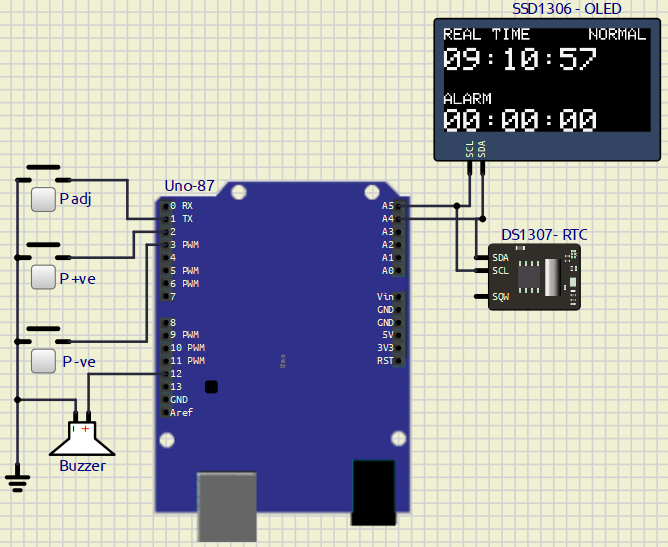
\includegraphics[width=0.50\textwidth]{Exp-4/Alarm_clock/Circuit.png}

\caption{Real-Time Alarm Clock Circuit Diagram}
\label{fig:alarm_clock}

\end{figure}

%%%%%%%%%%%%%%%%%%%%%%%%%%%%%%%%%%%%%%%%%%%%%%%%%%%%%%%%%%%%%%%%%%%%%%%

\subsection{Source Code}

The complete Arduino source code for this experiment is available in the project repository.

\href{https://github.com/YOUR_USERNAME/YOUR_REPOSITORY/blob/main/Exp-4/Alarm_Clock/alarm_clock.ino}
{\textbf{Click here to view the Arduino Source Code}}

%%%%%%%%%%%%%%%%%%%%%%%%%%%%%%%%%%%%%%%%%%%%%%%%%%%%%%%%%%%%%%%%%%%%%%%
%%%%%%%%%%%%%%%%%%%%%%%%%%%%%%%%%%%%%%%%%%%%%%%%%%%%%%%%%%%%%%%%%%%%%%%

\subsection{Working Principle}

\begin{enumerate}

\item The DS1307 RTC module continuously maintains the current date and time using its internal clock.

\item Arduino UNO communicates with the RTC module through the I\textsuperscript{2}C interface and reads the current time periodically.

\item The SSD1306 OLED display continuously shows:
\begin{itemize}
    \item Current Time
    \item Alarm Time
    \item Current Alarm Setting Mode
\end{itemize}

\item The \textbf{P-adj} button is used to change the alarm configuration mode.

\item The \textbf{P+ve} and \textbf{P-ve} buttons increase or decrease the selected alarm parameter (Hour, Minute, or Second).

\item The configured alarm hour, minute, and second are stored in memory.

\item When the current RTC time matches the configured alarm time:

\begin{itemize}
    \item The Arduino activates the buzzer.
    \item The buzzer sounds continuously to notify the user.
\end{itemize}

\item The alarm automatically stops when the current time changes beyond the configured alarm time.

\end{enumerate}

%%%%%%%%%%%%%%%%%%%%%%%%%%%%%%%%%%%%%%%%%%%%%%%%%%%%%%%%%%%%%%%%%%%%%%%

\subsection{Output}

\begin{figure}[H]
\centering

\begin{minipage}{0.31\textwidth}
\centering
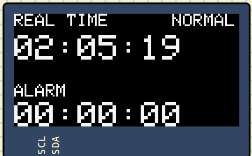
\includegraphics[width=\linewidth]{Exp-4/Alarm_clock/Realtime.png}
\\
\small (a) Real-Time Clock Display
\end{minipage}
\hfill
\begin{minipage}{0.31\textwidth}
\centering
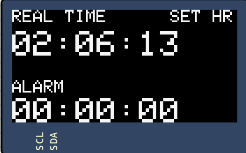
\includegraphics[width=\linewidth]{Exp-4/Alarm_clock/Alarm setting mode.png}
\\
\small (b) Alarm Setting Mode
\end{minipage}

\caption{Output of the Real-Time Alarm Clock System}
\label{fig:alarm_output}

\end{figure}

%%%%%%%%%%%%%%%%%%%%%%%%%%%%%%%%%%%%%%%%%%%%%%%%%%%%%%%%%%%%%%%%%%%%%%%

\subsection{Conclusion}

The Real-Time Alarm Clock using Arduino UNO, DS1307 RTC Module, SSD1306 OLED Display, push buttons, and a buzzer was successfully implemented and tested.

The system accurately displayed the current time, allowed users to configure alarm settings, and activated the buzzer when the current RTC time matched the preset alarm time. This experiment provided practical experience in real-time clock interfacing, OLED display programming, push-button handling, and alarm logic implementation in embedded systems.

During this experiment, the following concepts were learned:

\begin{itemize}

\item I\textsuperscript{2}C communication protocol

\item RTC interfacing

\item OLED display handling

\item Push-button interfacing

\item Alarm logic implementation

\item Embedded system programming

\end{itemize}

%%%%%%%%%%%%%%%%%%%%%%%%%%%%%%%%%%%%%%%%%%%%%%%%%%%%%%%%%%%%%%%%%%%%%%%

\subsection{References}

\begin{enumerate}

\item Arduino UNO Official Documentation

\url{https://docs.arduino.cc/hardware/uno-rev3/}

\item DS1307 RTC Module Documentation

\url{https://datasheets.maximintegrated.com/en/ds/DS1307.pdf}

\item RTClib Library Documentation

\url{https://github.com/adafruit/RTClib}

\item Adafruit SSD1306 OLED Library

\url{https://github.com/adafruit/Adafruit_SSD1306}

\item Adafruit GFX Graphics Library

\url{https://github.com/adafruit/Adafruit-GFX-Library}

\item I\textsuperscript{2}C Communication Protocol

\url{https://www.arduino.cc/en/reference/wire}

\end{enumerate}

%%%%%%%%%%%%%%%%%%%%%%%%%%%%%%%%%%%%%%%%%%%%%%%%%%%%%%%%%%%%%%%%%%%%%%%

\clearpage

%%%%%%%%%%%%%%%%%%%%%%%%%%%%%%%%%%%%%%%%%%%%%%%%%%%%%%%%%%%%%%%%%%%%%%%

\clearpage
Experiment 4 (Go Further 1):
\section{RTC-Based Water Supply Monitoring and Pump Status Display System}

%%%%%%%%%%%%%%%%%%%%%%%%%%%%%%%%%%%%%%%%%%%%%%%%%%%%%%%%%%%%%%%%%%%%%%%

\subsection{Problem Statement}

The objective of this project is to design and implement an automatic motor ON/OFF control system using Arduino UNO.

The system detects water supply using a switch sensor and controls a pump indicator LED based on water availability. A DS1307 Real-Time Clock (RTC) module is used for real-time tracking and timing operations, while an SSD1306 OLED display continuously shows the current time, water supply status, and pump status.

Additionally, the system monitors whether the water supply remains available continuously for more than one hour.

%%%%%%%%%%%%%%%%%%%%%%%%%%%%%%%%%%%%%%%%%%%%%%%%%%%%%%%%%%%%%%%%%%%%%%%

\subsection{Components Used \& Pin Connections}

\begin{table}[H]
\centering

\begin{minipage}[t]{0.48\textwidth}
\centering
\caption{Motor ON/OFF System Components}
\label{tab:motor_components}

\begin{tabular}{|p{4cm}|c|}
\hline
\textbf{Component} & \textbf{Quantity} \\
\hline
Arduino UNO & 1 \\
DS1307 RTC Module & 1 \\
SSD1306 OLED Display & 1 \\
Push Button / Water Sensor Switch & 1 \\
LED (Pump Indicator) & 1 \\
Breadboard & 1 \\
Jumper Wires & Required \\
\hline
\end{tabular}

\end{minipage}
\hfill
\begin{minipage}[t]{0.47\textwidth}
\centering
\caption{Water Sensor and Pump Connections}
\label{tab:motor_pins}

\begin{tabular}{|l|c|}
\hline
\textbf{Device} & \textbf{Arduino Pin} \\
\hline
Water Supply Switch & D2 \\
Pump Indicator LED & D3 \\
\hline
\end{tabular}

\end{minipage}

\end{table}

%%%%%%%%%%%%%%%%%%%%%%%%%%%%%%%%%%%%%%%%%%%%%%%%%%%%%%%%%%%%%%%%%%%%%%%

\subsection{RTC and OLED Connections}

\begin{table}[H]
\centering
\caption{RTC and OLED Connections}
\label{tab:motor_rtc}

\begin{tabular}{|l|c|}
\hline
\textbf{Device} & \textbf{Arduino Pin} \\
\hline
RTC VCC & 5V \\
RTC GND & GND \\
RTC SDA & A4 \\
RTC SCL & A5 \\
OLED VCC & 5V \\
OLED GND & GND \\
OLED SDA & A4 \\
OLED SCL & A5 \\
\hline
\end{tabular}

\end{table}

%%%%%%%%%%%%%%%%%%%%%%%%%%%%%%%%%%%%%%%%%%%%%%%%%%%%%%%%%%%%%%%%%%%%%%%

\subsection{Software Used}

\begin{itemize}
    \item Arduino IDE
    \item SimulIDE / Proteus
\end{itemize}

%%%%%%%%%%%%%%%%%%%%%%%%%%%%%%%%%%%%%%%%%%%%%%%%%%%%%%%%%%%%%%%%%%%%%%%

\subsection{Circuit Diagram}

\begin{figure}[H]
\centering

\begin{minipage}{0.48\textwidth}
\centering
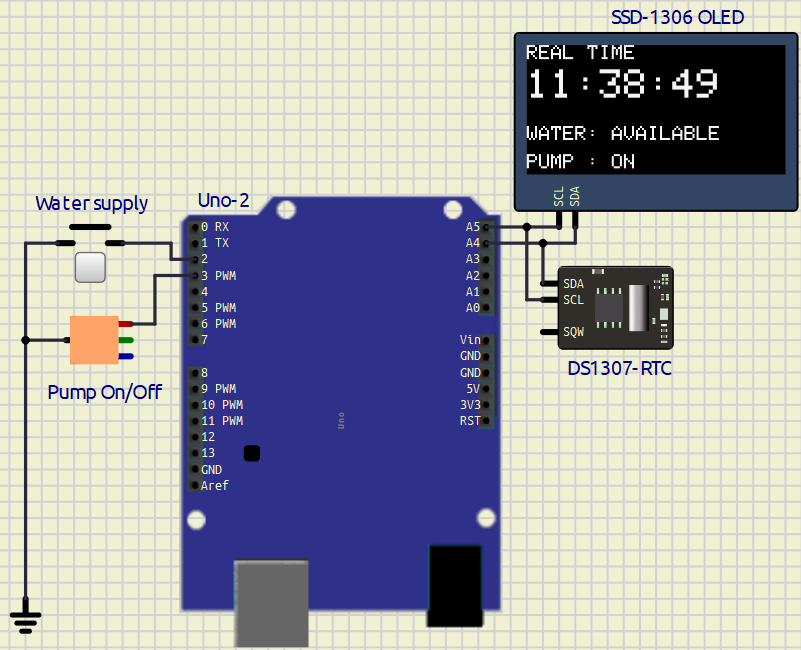
\includegraphics[width=\linewidth]{Exp-4/motor_On_off/Cicuit_On.png}
\caption*{(a) Water Supply Available}
\end{minipage}
\hfill
\begin{minipage}{0.48\textwidth}
\centering
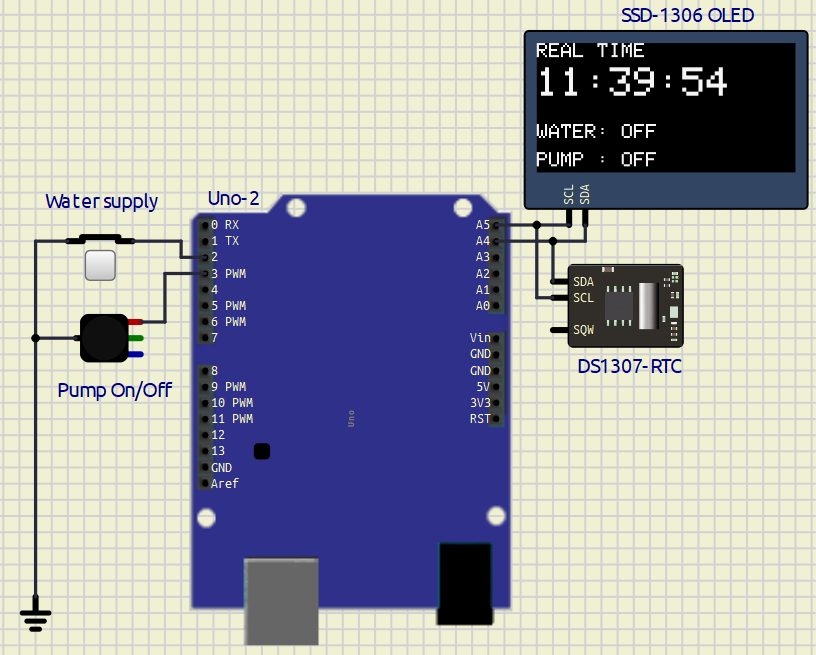
\includegraphics[width=\linewidth]{Exp-4/motor_On_off/Circuit_Off.png}
\caption*{(b) Water Supply OFF}
\end{minipage}

\caption{Alarm Based Motor ON/OFF System Circuit Diagrams}
\label{fig:motor_system}

\end{figure}

%%%%%%%%%%%%%%%%%%%%%%%%%%%%%%%%%%%%%%%%%%%%%%%%%%%%%%%%%%%%%%%%%%%%%%%

\subsection{Source Code}

The complete Arduino source code for this experiment is available in the project repository.

\href{https://github.com/YOUR_USERNAME/YOUR_REPOSITORY/blob/main/Exp-4/motor_On_off/file.ino}
{\textbf{Click here to view the Arduino Source Code}}

%%%%%%%%%%%%%%%%%%%%%%%%%%%%%%%%%%%%%%%%%%%%%%%%%%%%%%%%%%%%%%%%%%%%%%%
%%%%%%%%%%%%%%%%%%%%%%%%%%%%%%%%%%%%%%%%%%%%%%%%%%%%%%%%%%%%%%%%%%%%%%%

\subsection{Working Principle}

\begin{enumerate}

\item The water sensor continuously monitors the availability of water supply.

\item When water is available:

\begin{itemize}
    \item The pump indicator LED turns ON.
    \item The DS1307 RTC module records the starting time.
\end{itemize}

\item The Arduino continuously calculates the elapsed time using the RTC module.

\item If the water supply remains available continuously for more than one hour:

\begin{itemize}
    \item The predefined timer condition becomes true.
    \item Additional control logic can be implemented based on application requirements.
\end{itemize}

\item If the water supply is interrupted before one hour:

\begin{itemize}
    \item The system waits for two seconds.
    \item The pump indicator LED turns OFF.
    \item The timer is reset.
\end{itemize}

\item Throughout the operation, the SSD1306 OLED display continuously shows:

\begin{itemize}
    \item Current Real-Time Clock
    \item Water Supply Status
    \item Pump Status
\end{itemize}

\end{enumerate}


%%%%%%%%%%%%%%%%%%%%%%%%%%%%%%%%%%%%%%%%%%%%%%%%%%%%%%%%%%%%%%%%%%%%%%%

\subsection{Conclusion}

The Alarm Based Motor ON/OFF System using Arduino UNO, DS1307 RTC Module, and SSD1306 OLED Display was successfully implemented and tested.

The system accurately detected water supply conditions, controlled the pump indicator based on water availability, and continuously displayed the real-time status on the OLED display. The integration of RTC timing functionality further demonstrated the implementation of time-based monitoring and automation in embedded systems.

During this experiment, the following concepts were learned:

\begin{itemize}

\item RTC interfacing

\item OLED display interfacing

\item I\textsuperscript{2}C communication

\item Digital input/output control

\item Embedded automation logic

\end{itemize}

%%%%%%%%%%%%%%%%%%%%%%%%%%%%%%%%%%%%%%%%%%%%%%%%%%%%%%%%%%%%%%%%%%%%%%%

\subsection{References}

\begin{enumerate}

\item Arduino UNO Official Documentation

\url{https://docs.arduino.cc/hardware/uno-rev3/}

\item DS1307 RTC Datasheet

\url{https://datasheets.maximintegrated.com/en/ds/DS1307.pdf}

\item RTClib Library

\url{https://github.com/adafruit/RTClib}

\item Adafruit SSD1306 OLED Library

\url{https://github.com/adafruit/Adafruit_SSD1306}

\item Adafruit GFX Graphics Library

\url{https://github.com/adafruit/Adafruit-GFX-Library}

\item Arduino Wire Library Documentation

\url{https://www.arduino.cc/en/reference/wire}

\end{enumerate}

%%%%%%%%%%%%%%%%%%%%%%%%%%%%%%%%%%%%%%%%%%%%%%%%%%%%%%%%%%%%%%%%%%%%%%%

\clearpage

%%%%%%%%%%%%%%%%%%%%%%%%%%%%%%%%%%%%%%%%%%%%%%%%%%%%%%%%%%%%%%%%%%%%%%%

\clearpage
Experiment 4 (Go Further 2): 
\section{Temperature Data Logger Using I\textsuperscript{2}C Bus}

%%%%%%%%%%%%%%%%%%%%%%%%%%%%%%%%%%%%%%%%%%%%%%%%%%%%%%%%%%%%%%%%%%%%%%%

\subsection{Problem Statement}

The objective of this project is to design and implement a real-time temperature monitoring and recording system using Arduino UNO.

The system continuously measures ambient temperature using a DHT11 sensor and records the measured temperature values at regular intervals. A DS1307 Real-Time Clock (RTC) module provides accurate timestamps, while an SSD1306 OLED display continuously shows the current time, temperature, and EEPROM memory address.

The recorded temperature data is stored in the Arduino EEPROM and simultaneously transmitted to a laptop through USB serial communication for further analysis and logging.

%%%%%%%%%%%%%%%%%%%%%%%%%%%%%%%%%%%%%%%%%%%%%%%%%%%%%%%%%%%%%%%%%%%%%%%

\subsection{Components Used \& Pin Connections}

\begin{table}[H]
\centering

\begin{minipage}[t]{0.48\textwidth}
\centering
\caption{Temperature Data Logger Components}
\label{tab:logger_components}

\begin{tabular}{|p{4cm}|c|}
\hline
\textbf{Component} & \textbf{Quantity} \\
\hline
Arduino UNO & 1 \\
DHT11 Temperature Sensor & 1 \\
DS1307 RTC Module & 1 \\
SSD1306 OLED Display & 1 \\
Breadboard & 1 \\
USB Cable & 1 \\
Jumper Wires & Required \\
\hline
\end{tabular}

\end{minipage}
\hfill
\begin{minipage}[t]{0.47\textwidth}
\centering
\caption{DHT11 Sensor Connections}
\label{tab:dht_connections}

\begin{tabular}{|l|c|}
\hline
\textbf{DHT11 Pin} & \textbf{Arduino Pin} \\
\hline
DATA & D2 \\
VCC & 5V \\
GND & GND \\
\hline
\end{tabular}

\end{minipage}

\end{table}

%%%%%%%%%%%%%%%%%%%%%%%%%%%%%%%%%%%%%%%%%%%%%%%%%%%%%%%%%%%%%%%%%%%%%%%

\subsection{RTC and OLED Connections}

\begin{table}[H]
\centering
\caption{RTC and OLED Connections}
\label{tab:logger_connections}

\begin{tabular}{|l|c|}
\hline
\textbf{Device} & \textbf{Arduino Pin} \\
\hline
RTC SDA & A4 \\
RTC SCL & A5 \\
RTC VCC & 5V \\
RTC GND & GND \\
OLED SDA & A4 \\
OLED SCL & A5 \\
OLED VCC & 5V \\
OLED GND & GND \\
\hline
\end{tabular}

\end{table}

%%%%%%%%%%%%%%%%%%%%%%%%%%%%%%%%%%%%%%%%%%%%%%%%%%%%%%%%%%%%%%%%%%%%%%%

\subsection{Software Used}

\begin{itemize}
    \item Arduino IDE
    \item SimulIDE
\end{itemize}

%%%%%%%%%%%%%%%%%%%%%%%%%%%%%%%%%%%%%%%%%%%%%%%%%%%%%%%%%%%%%%%%%%%%%%%

\subsection{Circuit Diagram}

\begin{figure}[H]
\centering

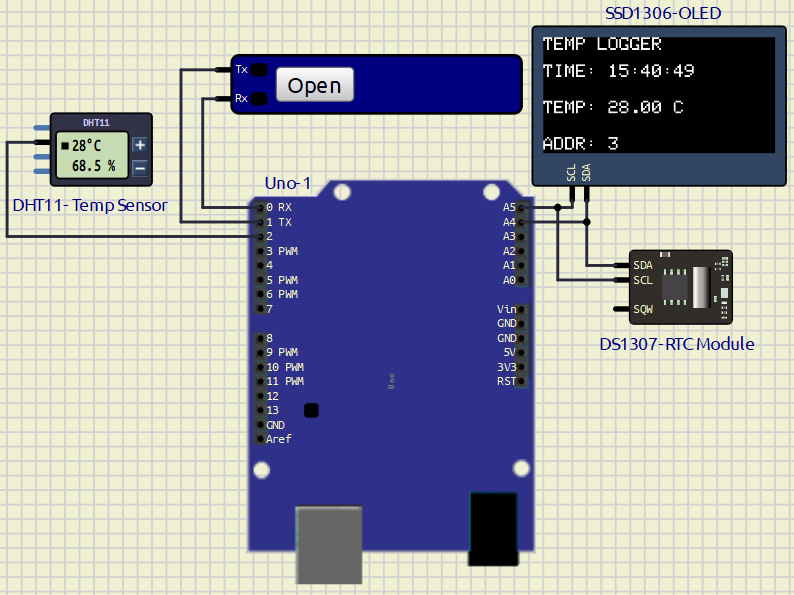
\includegraphics[width=0.80\textwidth]{Exp-4/temp_recorder/circuit.png}

\caption{Temperature Data Logger Circuit Diagram}
\label{fig:temp_logger}

\end{figure}

%%%%%%%%%%%%%%%%%%%%%%%%%%%%%%%%%%%%%%%%%%%%%%%%%%%%%%%%%%%%%%%%%%%%%%%

\subsection{Source Code}

The complete Arduino source code for this experiment is available in the project repository.

\href{https://github.com/YOUR_USERNAME/YOUR_REPOSITORY/blob/main/Exp-4/temp_recorder/file.ino}
{\textbf{Click here to view the Arduino Source Code}}

%%%%%%%%%%%%%%%%%%%%%%%%%%%%%%%%%%%%%%%%%%%%%%%%%%%%%%%%%%%%%%%%%%%%%%%
%%%%%%%%%%%%%%%%%%%%%%%%%%%%%%%%%%%%%%%%%%%%%%%%%%%%%%%%%%%%%%%%%%%%%%%

\subsection{Working Principle}

\begin{enumerate}

\item The DHT11 sensor continuously measures the ambient temperature.

\item The DS1307 RTC module continuously maintains the current date and time using the I\textsuperscript{2}C communication protocol.

\item Arduino UNO periodically reads:

\begin{itemize}
    \item Current temperature from the DHT11 sensor.
    \item Current time from the DS1307 RTC module.
\end{itemize}

\item The SSD1306 OLED display continuously shows:

\begin{itemize}
    \item Current Time
    \item Current Temperature
    \item EEPROM Memory Address
\end{itemize}

\item At every predefined recording interval (15 minutes), Arduino:

\begin{itemize}
    \item Stores the current time and temperature in the internal EEPROM.
    \item Updates the EEPROM memory address.
    \item Sends the recorded data to the laptop through USB serial communication.
\end{itemize}

\item The Serial Monitor continuously displays the recorded temperature log with the corresponding timestamp.

\item In this implementation, the recording interval was modified to one minute instead of fifteen minutes for demonstration purposes.

\end{enumerate}

%%%%%%%%%%%%%%%%%%%%%%%%%%%%%%%%%%%%%%%%%%%%%%%%%%%%%%%%%%%%%%%%%%%%%%%

\subsection{Output}

%%%%%%%%%%%%%%%%%%%%%%%%%%%%%%%%%%%%%%%%%%%%%%%%%%%%%%%%%%%%%%%%%%%%%%%

\subsubsection*{Serial Monitor Output}

\begin{figure}[H]
\centering
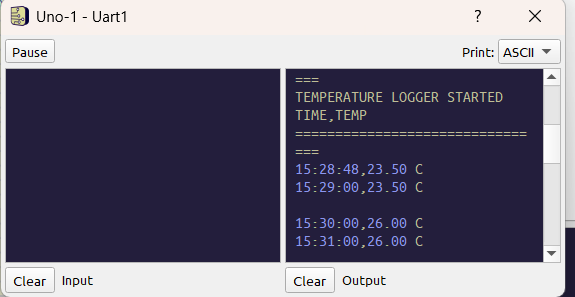
\includegraphics[width=0.75\textwidth]{Exp-4/temp_recorder/Serial monitor.png}
\caption{Recorded Temperature Data Displayed on the Serial Monitor}
\label{fig:temp_logger_serial}
\end{figure}

%%%%%%%%%%%%%%%%%%%%%%%%%%%%%%%%%%%%%%%%%%%%%%%%%%%%%%%%%%%%%%%%%%%%%%%

\subsection{Conclusion}

The Temperature Data Logger using Arduino UNO, DHT11 Sensor, DS1307 RTC Module, and SSD1306 OLED Display was successfully implemented and tested.

The system continuously monitored temperature, displayed live information on the OLED screen, stored periodic temperature records in the Arduino EEPROM, and transferred the recorded data to a laptop through USB serial communication. This project demonstrated an effective and low-cost embedded data logging solution.

During this experiment, the following concepts were learned:

\begin{itemize}

\item RTC interfacing

\item OLED display interfacing

\item EEPROM memory management

\item Serial communication

\item Temperature sensing

\item Embedded data logging techniques

\end{itemize}

%%%%%%%%%%%%%%%%%%%%%%%%%%%%%%%%%%%%%%%%%%%%%%%%%%%%%%%%%%%%%%%%%%%%%%%
\clearpage
\subsection{References}

\begin{enumerate}

\item Arduino UNO Official Documentation

\url{https://docs.arduino.cc/hardware/uno-rev3/}

\item DHT11 Sensor Documentation

\url{https://components101.com/sensors/dht11-temperature-sensor}

\item DS1307 RTC Datasheet

\url{https://datasheets.maximintegrated.com/en/ds/DS1307.pdf}

\item RTClib Library

\url{https://github.com/adafruit/RTClib}

\item Adafruit SSD1306 OLED Library

\url{https://github.com/adafruit/Adafruit_SSD1306}

\item EEPROM Library Documentation

\url{https://www.arduino.cc/en/Reference/EEPROM}

\end{enumerate}

%%%%%%%%%%%%%%%%%%%%%%%%%%%%%%%%%%%%%%%%%%%%%%%%%%%%%%%%%%%%%%%%%%%%%%%

\clearpage